\documentclass{sig-alternate}

\begin{document}

\title{Seguimiento de un blanco m\'{o}vil}

\numberofauthors{2}

\author{
    \alignauthor
    Villa Fern\'{a}ndez, Santiago\\
    \email{svillafe@alu.itba.edu.ar} \\
    \ \\
    Gomez Vidal, Maximiliano\\
    \email{dgomezvi@alu.itba.edu.ar} \\
    \alignauthor
    Sessa, Carlos\\
    \email{csessa@alu.itba.edu.ar} \\
    \ \\
    Abramowicz, Pablo\\
    \email{pabramow@alu.itba.edu.ar} \\
}

\maketitle

\begin{abstract}
En este art\'{i}culo se modela un sistema de seguimiento de blancos a lazo 
cerrado. Se analiza el comportamiento del sistema con distintos tipos de \
controladores: proporcional, integral y derivativo.
\end{abstract}

\keywords{Seguimiento de blancos, sistema de control, controlador proporcional,
controlador derivativo, controlador integral}

\section{Introducci\'{o}n}\label{introduccion}
Un sistema de seguimiento de blancos consiste en un radar y una antena.
Se desea que la antena apunte al blanco, por lo que se debe ajustar su 
posici\'{o}n  seg\'{u}n corresponda. Para esto se incluye un controlador que 
compara el \'{a}ngulo de la antena con el \'{a}ngulo en donde se encuentra el 
objetivo y proporciona el torque correspondiente para minimizar la discrepancia 
entre ambos.

En la secci\'{o}n \ref{modelo} se describe el modelo del sistema. En la
secci\'{o}n \ref{simulaciones} se realizan las simulaciones correspondientes
a los tres tipos de controladores utilizados: proporcional, integral y 
derivativo. Por \'{u}ltimo, se exponen las conclusiones en la secci\'{o}n
\ref{conclusiones}.

\section{Modelo}\label{modelo}
La din\'{a}mica de la antena se modela seg\'{u}n la ecuaci\'{o}n diferencial:
\begin{equation}
\label{dinamica_antena}
I \ddot\theta = - b \dot\theta + u(t)
\end{equation}
donde $\theta$ es el \'{a}ngulo que corresponde a la direcci\'{o}n en la que
apunta el radar, $I$ es el momento de inercia de la antena y $b$ es una 
constante positiva que vincula la fuerza viscosa que act\'{u}a sobre la antena.
El torque que producen los motores sobre la antena est\'{a} representado por 
la funci\'{o}n $u$.

Se desea que el sistema sea a lazo cerrado. Para esto se mide el \'{a}ngulo
$\theta$ de la antena y se lo compara con el \'{a}ngulo $\theta_{R}$ que marca
la ubicaci\'{o}n real del objetivo. La diferencia entre ambos constituye una
se\~{n}al de error $e(t) = \theta_{R}(t) - \theta(t)$ que se ingresa nuevamente 
al controlador.

\section{Simulaciones}\label{simulaciones}
Para realizar la simulaci\'{o}n se consideran los par\'{a}metros 
$I = 0.004\ kg\ m^{2}$ y $b = 0.02\ kg\  m^{2}\ s^{-1}$. Tambi\'{e}n se establece
que el blanco se mueve de acuerdo a $\theta_{R}(t) = 0.01 t$.
Se estudian tres tipos de controladores: proporcional, integral y derivativo.
En todos los casos se utiliza el m\'{e}todo de Runge-Kutta de orden $4$ para
la resoluci\'{o}n num\'{e}rica de las ecuaciones diferenciales.

\subsection{Controlador proporcional}\label{proporcional}
%TODO: explicar modelo proporcional

\subsection{Controlador integral}\label{integral}
%TODO: explicar modelo integral

\subsection{Controlador derivativo}\label{derivativo}
%TODO: explicar modelo derivativo

\section{Conclusiones}\label{conclusiones}
A partir de las simulaciones se observa que el controlador proporcional es el
m\'{a}s estable y preciso de los tres controladores analizados. El
controlador integral resulta sumamente inestable, presentando oscilaciones
que aumentan su amplitud con el paso del tiempo. Para determinados casos puede
utilizarse un controlador derivativo, aunque depender\'{a} de los par\'{a}metros
del radar, pues resulta menos efectivo que el proporcional.

\begin{figure*}[hp]
\label{mProporcional}
\centering
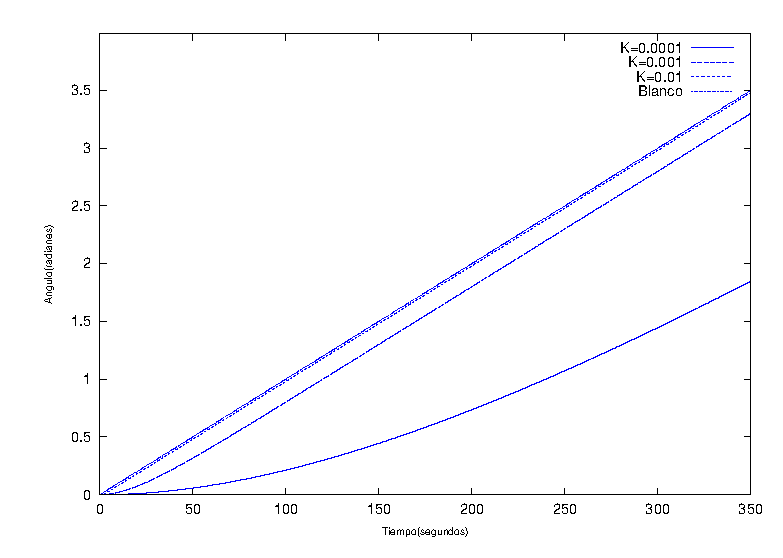
\includegraphics[scale=0.8]{graficos/mProporcional}
\caption{Salida $\theta(t)$ con controlador proporcional}
\end{figure*}

\begin{figure*}[hp]
\label{mIntegral}
\centering
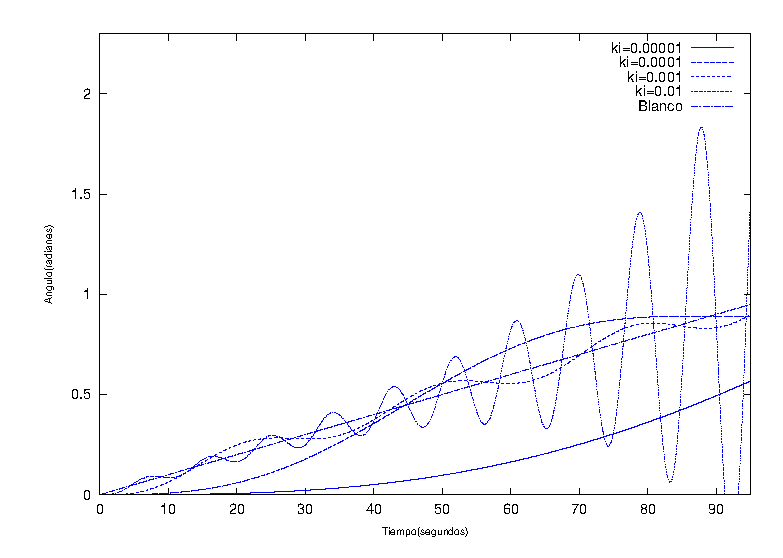
\includegraphics[scale=0.8]{graficos/mIntegral}
\caption{Salida $\theta(t)$ con controlador integral}
\end{figure*}

\begin{figure*}[hp]
\label{mDerivativo}
\centering
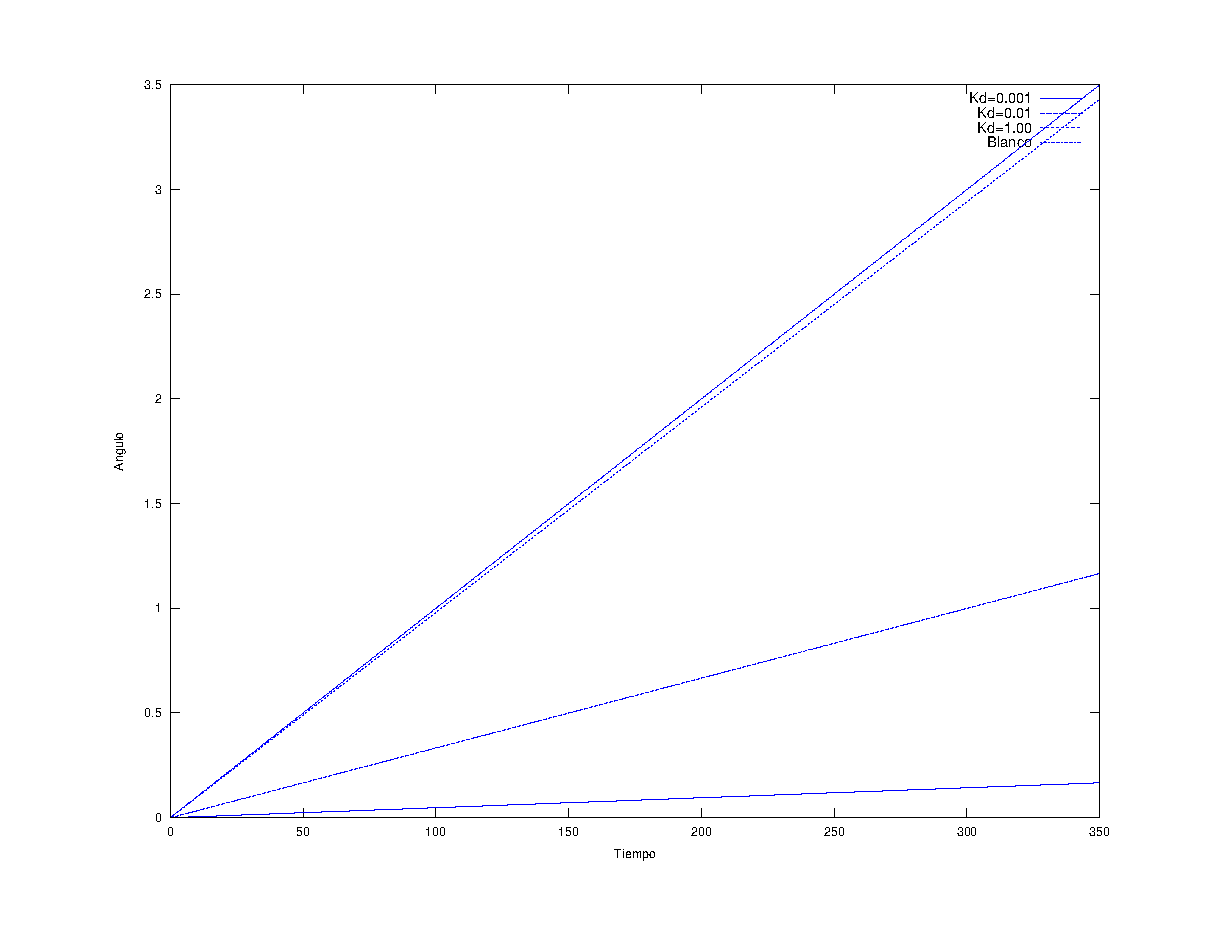
\includegraphics[scale=0.8]{graficos/mDerivativo}
\caption{Salida $\theta(t)$ con controlador derivativo}
\end{figure*}

\begin{figure*}[hp]
\label{errorMProporcional}
\centering
\includegraphics[scale=0.8]{graficos/errorMProporcional}
\caption{Error relativo porcentual al utilizar un controlador proporcional}
\end{figure*}

\begin{figure*}[hp]
\label{errorMIntegral}
\centering
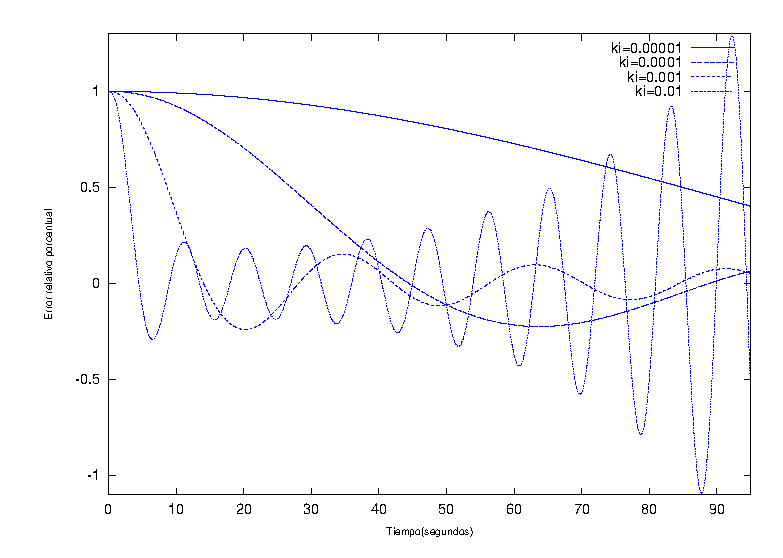
\includegraphics[scale=0.8]{graficos/errorMIntegral}
\caption{Error relativo porcentual al utilizar un controlador integral}
\end{figure*}

\begin{figure*}[hp]
\label{errorMDerivativo}
\centering
\includegraphics[scale=0.8]{graficos/errorMDerivativo}
\caption{Error relativo porcentual al utilizar un controlador derivativo}
\end{figure*}
\end{document}
